% Template for 61st conference for non-peer-reviewed articled
\documentclass[convention,peer-reviewed]{aesconf}

% Graphics path
\graphicspath{{./}{figs/}}

% UTF-8 encoding is recommended but use one that works for you.
\usepackage[utf8]{inputenc}

% Highly recommended package for better looking text automatically.
\usepackage{microtype}

% Natbib is used for more control on citations. You can use other moderd
% bibliography packages but please try to match the provided style.
\usepackage[numbers,square]{natbib} 


% These are useful for different purposes.
\usepackage{color}
\usepackage{url}
\usepackage{colortbl}
\usepackage{graphicx}
\usepackage{amsmath}
\DeclareMathOperator*{\argmin}{arg\,min}
\DeclareMathOperator*{\argmax}{arg\,max}
\usepackage{multirow}
\usepackage{rotating}
\usepackage{setspace}
\usepackage{subfigure}
\usepackage{svg}

% The full title of the paper
\title{Automatic Guitar Tablature Transcription from Audio using Inharmonicity Regressions
and Bayesian Classification}

% Put the authors in order here. The number in brackets define the corresponding affiliation.
\author[1]{Jonathan Michelson}
\author[2]{Richard Stern}
\author[2]{Thomas Sullivan}

% Affiliations go here
\affil[1]{Electro-Harmonix / New Sensor Corporation}
\affil[2]{Carnegie Mellon University}

% Correspondece should include the corresponding author's name and e-mail address
\correspondence{Jonathan Michelson}{jonathan@ehx.com}

% These are used for headers. Anything that fits is okay. Please use proper punctuation.

% If there are many authors, please use the form "First author et al."
\lastnames{Michelson et al.}

% Short title should describe your topic but not be too long.
\shorttitle{Tablature Transcription using Inharmonicity Regressions}


% This is required and draws the top title
% AES top title. A little bit volatile but should work for now.
\savebox{\AEStop}{%
	\begin{minipage}{\textwidth}%
		\rule{\textwidth}{1.5pt}\\%
		\\%
		\begin{minipage}[c][\iftoggle{convention}{3.2cm}{3.7cm}][t]{0\textwidth}%
			\includegraphics[width=20mm]{AESlogo}%
		\end{minipage}%
		\begin{minipage}{\textwidth}%
			\sffamily%
			\begin{center}%
				\LARGE Audio Engineering Society\\%
				\iftoggle{e_brief}{%
				\hspace{3mm}\fontsize{36}{38pt}\selectfont Convention e-Brief \AESEBriefNumber\\%
				}{%
				\iftoggle{convention}{%
				\fontsize{36}{38pt}\selectfont Convention Paper\\%
				}{%
				\fontsize{36}{38pt}\selectfont Conference Paper\\%
				}}%
				\vspace{0.2cm}%
				\large Presented at the \AESConferenceNumber \iftoggle{convention}{Convention\\}{Conference on\\}%
				\iftoggle{convention}{}{\AESConferenceTopic\\}%
				\AESConferenceDate, \AESConferenceLocation%
			\end{center}%
		\end{minipage}\\%
		\vspace{0.2cm}\\%
		\begin{minipage}{\textwidth}%
			\rmfamily\itshape\small	\AESLegalText%
		\end{minipage}\\%
		\\%
		\rule{\textwidth}{1.5pt}%
	\end{minipage}%
}

\begin{document}


\twocolumn[
\maketitle % MANDATORY! 

\begin{onecolabstract}
We propose two new methods to classify guitar strings using only audio with the goal of developing automated tablature transcription. The first method regresses the log-inharmonicities of guitar strings against their pitches to obtain characteristic linear trajectories, and assigns unseen notes to the strings of the regressions whose means and variances maximize the probability of the measured inharmonicities of the notes. The second method, developed as a baseline against which to measure the first, characterizes the inharmonicity distribution of each fretboard position as a normal probability density, then similarly assigns unseen notes to the fretboard positions that maximize the likelihood of their observed inharmonicities. Results from the standard Real World Corpus of guitar recordings show that exploiting log-inharmonicity regressions generally increases performance compared to our Bayesian method, but does not generally increase performance on classical and acoustic guitars compared to the existing inharmonicity-based system in \citep{barbanchoi2012}. Also in this work, we derive an inharmonicity compensation feature to allow for transcription of arbitrarily-tuned guitars, provided the tuning is known. Results from personally-recorded acoustic and electric guitars in various alternate tunings show that our tuning compensation is successful at predicting tuning-related inharmonicity changes.
\end{onecolabstract}
]

\section{Introduction}

The guitar is a popular musical instrument whose family comprises a diverse collection of stringed instruments. Despite their variation, the majority of guitar configurations exhibit six strings tuned to $E2$ ($82$ Hz), $A2$ ($110$ Hz), $D3$ ($147$ Hz), $G3$ ($196$ Hz), $B3$ ($247$ Hz), and $E4$ ($330$ Hz). Most guitars also typically have upwards of 20 frets, allowing for versatile musical passage realizations along the fretboard. A consequence of the tuning and extensive fretting locations is liberal pitch overlap between neighboring strings; multiple fretboard locations can usually be selected to produce a given pitch. This ambiguity renders conventional music scores, which represent passages as notes and chords, undesirable for students trying to learn more skillful placement of scales and arpeggios, or for enthusiasts trying to uncover the fretboard positions used on riffs recorded by virtuosic players. Figure~\ref{fig:score-tabs} illustrates this ambiguity.

Tablature is a desirable, alternative music notation that does not suffer from the one-to-many mapping of scores. The staff, instead of representing pitch as in classical notation, depicts a birds-eye view of the guitar neck from the perspective of the performer. Each of the six horizontal lines signify a corresponding string on the guitar, and numbers on each line specify the fret to be fingered. Reasons for tablature desirability are numerous \citep{macrae2010}, such as accessibility (legibility does not require formal musical training) and transportability (tablature can be easily represented with ASCII characters). 

Accurate tablature transcription is a laborious task, however. Dependable tablature containing few errors typically require the careful listening of a seasoned musician to an audio recording, and possibly video recordings for additional consultation. Reliable automation of this transcription task would benefit the guitar student community by expediting quality tablature generation and unearthing fretboard positions of guitar riffs in songs for which accurate tablature does not yet exist.
\begin{figure}[!htbp] 
\centering
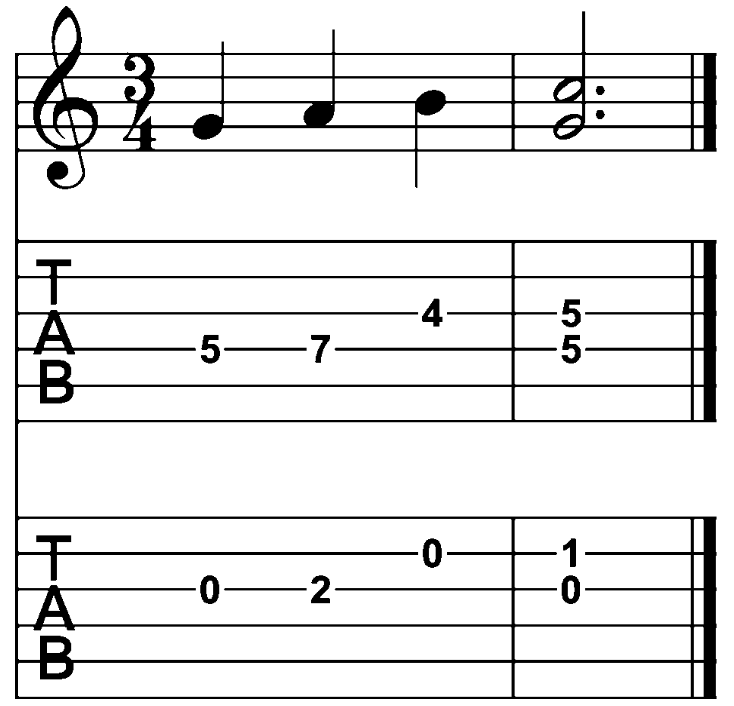
\includegraphics[scale=0.2]{figs/score-tabs}
\caption{Musical score and two identical realizations of that score in tablature notation. Figure taken from \citep{barbanchoi2012}.}
\label{fig:score-tabs}
\end{figure}

An important feature in systems that transcribe tablature from audio input is inharmonicity. When an ideal string fixed at both ends is displaced, the restoring force that causes it to oscillate is its tension. For a real string with stiffness, however, its elasticity contributes to this restoring force \citep{fletcher1962}, causing the frequencies of the modes of vibration to deviate from integer multiples of the fundamental. Instead, the solutions to the one-dimensional wave equation become: 
\begin{equation}
\label{eq:fk}
f_k = kf_{0}\sqrt{1+\beta k^2}
\end{equation}
where $f_k$ is the $k$th harmonic of fundamental $f_0$ and $\beta$ is the inharmonicity of the string, defined by
\begin{equation}
\beta = \frac{\pi^3 Q d^4}{64 T l^2}. \label{eq:beta}
\end{equation}
In other words, the inharmonicity $\beta$ of a vibrating string is a dimensionless quantity that depends on the Young's modulus $Q$, diameter $d$, tension $T$, and vibrating length $l$ of the string, and which skews the $k$th partial of the string upwards in frequency according to equation~(\ref{eq:fk}). See Figure~\ref{fig:skew}. 

\begin{figure}[!htbp]
\centering
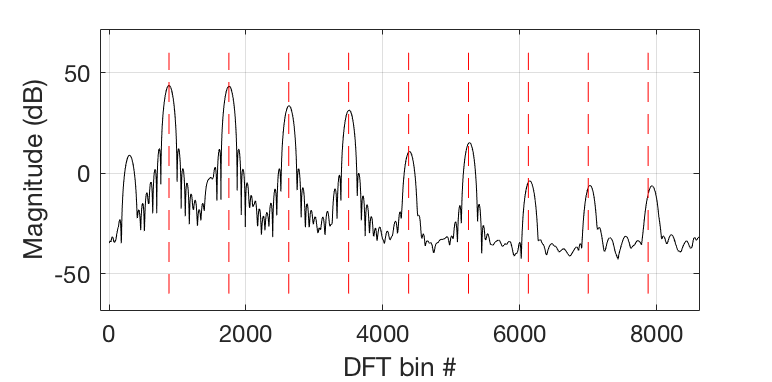
\includegraphics[scale=0.3]{skew}
\caption{Power spectrum of note D2 plucked on an electric guitar at string 5 and fret 5. Red dashed lines are drawn at integer multiples of the fundamental. The partial peaks begin visibly skewing rightward after the fifth harmonic.}
\label{fig:skew}
\end{figure}

Moreover, inharmonicity in the guitar varies in a deterministic manner with respect to fret positions along a given string \citep{barbanchoi2012}. Specifically, the inharmonicity $\beta(s,n)$ of a note produced by string $s$ at fret number $n$ can be expressed in terms of the inharmonicity of the open-string note $\beta(s,0)$ according to:
\begin{equation} 
\label{eq:beta-traj}
\beta(s,n) = \beta(s,0)2^{\frac{n}{6}}
\end{equation}
Figure~\ref{fig:beta-trajectories-ag} illustrates these trajectories. One existing transcription system \citep{barbanchoi2012} has successfully exploited this theoretical trajectory.

\begin{figure}[h] 
\centering
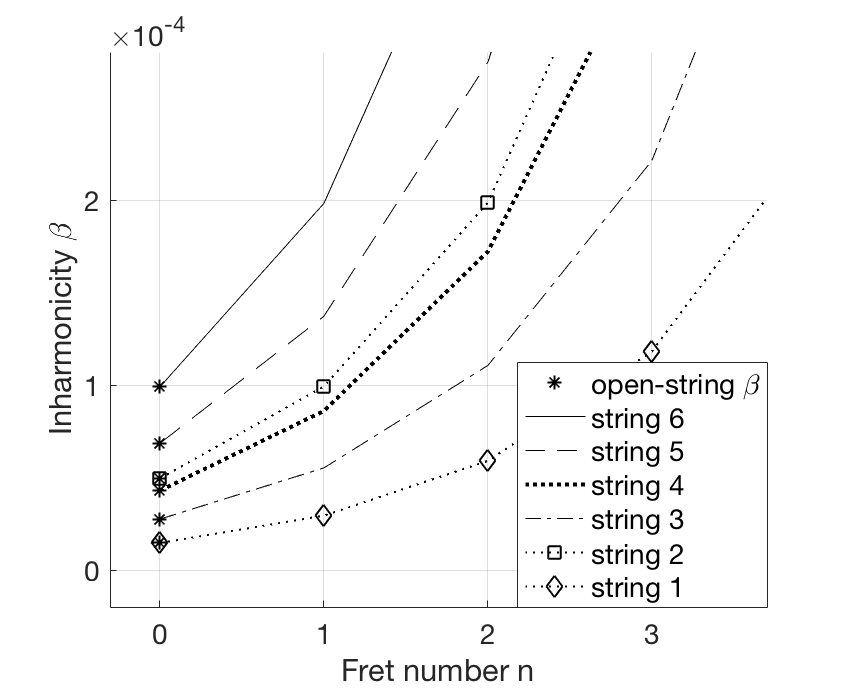
\includegraphics[scale=0.25]{figs/beta-trajectories-ag}
\caption{Example inharmonicity trajectories of acoustic guitar strings, calculated from measured open-string inharmonicities. Only Fret 0 (open-string) through Fret 3 are shown. Observe the restriction to the exponential trajectory defined by equation~\eqref{eq:beta-traj}.}
\label{fig:beta-trajectories-ag}
\end{figure}

Exploiting the \textit{empirical} trajectories of guitar strings, however, has not yet been investigated. If a sufficiently diverse set of guitars is sampled, the empirical trajectories may further increase transcription performance or improve system generalizability. We classify unseen notes as belonging to the string whose pre-computed log-inharmonicity regression most probably predicts the estimated log-inharmonicity of the note. To contextualize its performance as well as that of its predecessor, we also introduce a baseline Bayesian classifier of fretboard position given an unseen note: the measured inharmonicities of each fretboard position are collected and fit to a normal distribution, and are used to return the string that maximizes the probability of having observed the measured inharmonicity of the unseen note.

\section{Previous Work}

Empirical estimation of inharmonicity has been under investigation for nearly 40 years. Using pitch extraction techniques to perform estimation was first attempted by Galembo in 1979 and 1986 \citep{galembo1979,galembo1987}. Several additional methods have been proposed since then. In 1994, Galembo \citep{galembo1994} hypothesized a connection between partials-based fundamental pitch estimates and the degree of inharmonicity in a spectrum. They specifically investigated cepstral analysis and a variant of the harmonic product spectrum method applied to both synthetic tones and recorded piano notes. The same authors in \citep{galembo1999} introduced another method in 1999, dubbed the inharmonic comb filter (ICF) method. The ICF whose inharmonicity best matched that of the note would produce the output with lowest spectral energy, since its notches would most align with, and therefore best cancel, the inharmonic note partials. Rauhala \citep{rauhala2007} introduced an efficient procedure in 2007, known as partial frequency deviations (PDF), that iteratively catalogued estimates of the deviations of partial frequencies of a note and returned increasingly better estimates of the inharmonicity. In 2009, Hodgkinson \citep{hodgkinson2009} proposed a yet more efficient and accurate algorithm, named median-adjustive trajectories (MAT). Three years later, Barbancho \citep{barbanchoi2012} introduced another PFD-based approach, which we refer to as the partial coincidence tally (PCT) method, as part of a guitar tablature transcription system. Also in 2012, Abesser \citep{abesser2012} used parametric spectral modeling, again in the context of a guitar tablature transcription system.

Tablature transcription is also a rich research topic. A popular framework for the stringed-instrument transcription problem is that of weighted directed graphs that capture all plausible sequences of fretboard positions in a given musical passage \citep{sayegh1989,radicioni2005,yazawa2013,burlet2013,burlet2015,radisav2004}. A number of teams have had success with machine learning techniques such as neural networks, genetic algorithms, hidden Markov models, and SVMs  \citep{gagnon2003,tuohy2006,barbancho2009,barbanchoa2012,abesser2012,kehling2014,dittmar2013,abesser2012}. Some researchers have explored usage of media other than audio or musical information (i.e., scores), such as augmented guitar hardware and video recordings \citep{ogrady2009,paleari2008,kerd2007}.

\section{Methods}

\subsection{Inharmonicity Regression}
First, we estimate the inharmonicity of an unseen note. The algorithm we employ is the median adjustive trajectories (MAT) method \citep{hodgkinson2009} proposed by Hodgkinson in 2009. The MAT algorithm was chosen for its efficiency and accuracy over the algorithms that preceded it \citep{hodgkinson2009}. We apply this estimation procedure to five Hann-windowed audio segments of length $2^{14}$ samples, beginning at the detected onset of a note and at four successive 100-ms intervals (i.e. 0 ms, 100 ms, 200 ms, 300 ms, and 400 ms after the note onset). This yields five inharmonicity estimates we later compile into one classification result using the frame aggregation refinement technique in \citep{abesser2012}.

Next, we apply a log transformation to the estimated inharmonicities to make their variation linear with respect to MIDI pitch. If we reconsider equation~\eqref{eq:beta-traj} in terms of MIDI pitch number $m$ instead of fret number $n$, we obtain
\begin{equation}
\beta(s,m) = \beta(s,m_{os})2^{\frac{m-m_{os}}{6}},
\end{equation}
where $m_{os}$ is the open-string pitch of string $s$. Figure~\ref{fig:beta-v-midi} illustrates the trajectories in terms of MIDI pitches.
\begin{figure}[h] 
\centering
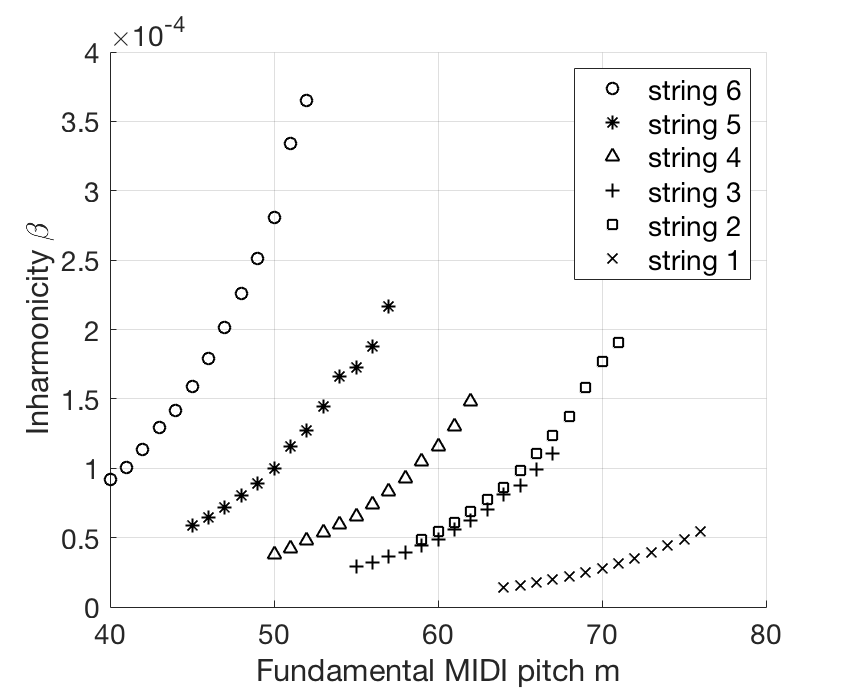
\includegraphics[scale=0.25]{beta-v-midi}
\caption{Inharmonicity estimates for Frets 0-12 on Strings 1-6 of RWC Acoustic Guitar AG111. Note the exponential trajectory as in Fig.~\ref{fig:beta-trajectories-ag} and the increased segregation since notes and their inharmonicities are now plotted against their fundamental instead of their fret number.}
\label{fig:beta-v-midi}
\end{figure}
Now if we consider the log-inharmonicity $\beta_{l}(m)$, we see that
\begin{equation}
\beta_l(m) = \log_2\beta(s,m) = \log_2[\beta(m_{os})2^{\frac{m-m_{os}}{6}}]
\end{equation}
\begin{equation}
\beta_l(m) = \log_2\beta(m_{os}) + \frac{m-m_{os}}{6}
\end{equation}
\begin{equation}
\beta_l(m) = (\log_2\beta(m_{os})-\frac{m_{os}}{6}) + (\frac{1}{6})m,
\end{equation}
where string $s$ has been dropped from the notation since we're looking only at variation along a fixed string. Substituting $w_0$ for $\log_2\beta(m_{os})-\frac{m_{os}}{6}$ and letting $w_1 = \frac{1}{6}$, we obtain the standar linear form
\begin{equation}
\label{eq:linear-traj}
\beta_l(m) = w_0 + w_1m,
\end{equation}
showing us that the log-inharmonicity trajectory of a given string varies linearly with respect to both MIDI pitch and fret number. See Figure~\ref{fig:log-beta-v-midi}.
\begin{figure}[!htbp] 
\centering
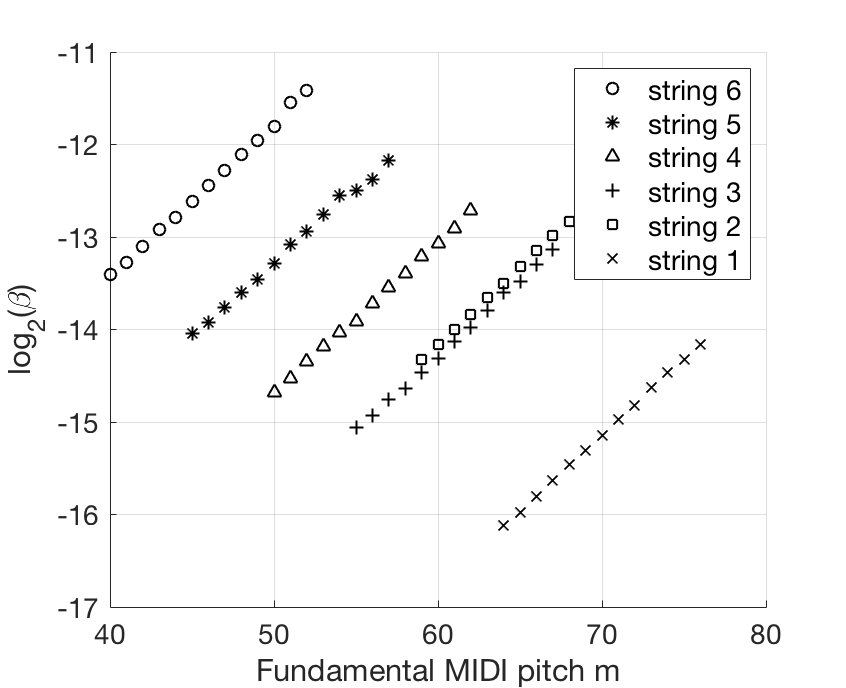
\includegraphics[scale=0.25]{log-beta-v-midi}
%\includesvg{figs/log-beta-v-midi}
\caption{Log-inharmonicity estimates for same frets, strings, and guitar as Fig.~\ref{fig:beta-v-midi}.}
\label{fig:log-beta-v-midi}
\end{figure}

We next use linear regressions to obtaining empirical log-inharmonicity trajectories in order to train our system to understand the typical trajectories of guitar strings. We collect all notes with common string labels in our training data, and we perform linear regression of their log-inharmonicities $\beta$ against their fundamental pitches $m$ (in MIDI note number format). We do this for each string label. Let $s \in \{1,2,3,4,5,6\}$ be the string label to which each training note is assigned, and $N_s$ be the number of notes we have belonging to string label $s$. If we let $\mathbf{x}_s^{(i)} = [1, m_s^{(i)}]^T$ represent the $i$th note with fundamental pitch $m^{(i)}_s$ belonging to string $s$ , and let $\beta_s^{(i)}$ denote the log-inharmonicity of the $i$th note belonging to string $s$, we can solve
\begin{equation}
\label{lin-reg}
\mathbf{w}_s = \argmin_{\mathbf{w}}{\sum_{i=1}^{N_s}{(\beta^{(i)}_s - \mathbf{w}^T\mathbf{x}^{(i)}_s)^2}}
\end{equation}
which yields the weight vector $\mathbf{w}_s$ that minimizes the sum of squared error between the measured and predicted inharmonicities of the notes belonging to string $s$.
%\begin{figure}[!htbp] 
%\centering
%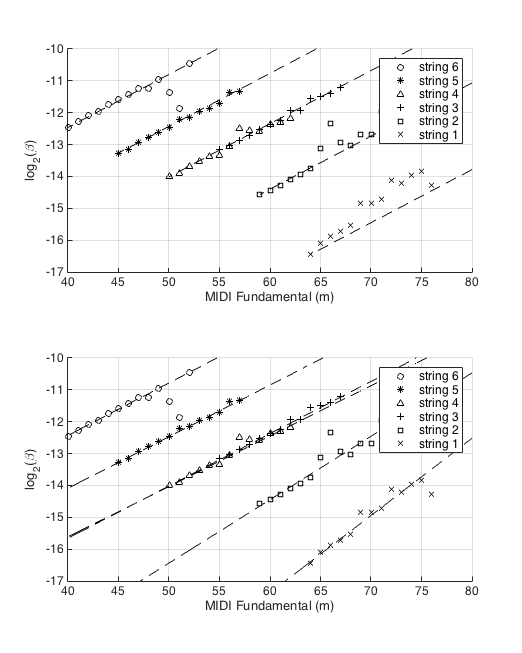
\includegraphics[scale=0.75]{traj-v-reg}
%\caption{Comparison of string inharmonicity characterization approaches for our recorded Fender Telecaster. Top: \textit{theoretical} trajectories. Note how each line begins precisely at the first marker of each string (i.e. the open-string note) and continues along a trajectory that ignores empirical inharmonicity estimates. String 1 most clearly shows this. Additionally, the trajectories for String 3 and String 4 are effectively co-linear and therefore indiscriminable. Bottom: regressions, or \textit{empirical} trajectories. Each regression was obtained by minimizing the bisquare weighted error of the residuals of the string, so the lines more closely follow the empirical inharmonicity scatterplot estimates.}
%\label{fig:traj-v-reg}
%\end{figure}

Occasional estimates from the inharmonicity measurement routine are outliers that deviate substantially from the linear trajectory model, so instead of the standard unweighted regression in~\eqref{lin-reg} we rather perform a bisquare weighted linear regression to approximate the log-inharmonicities. Bisquare weighting is a robust linear regression procedure that minimizes a \textit{weighted} sum of squares which de-emphasizes outliers \citep{matlab-robustfit}. This provides us with higher-quality regressions that were more robust to stray inharmonicity measurements.

To classify unknown notes, we impose Gaussian probability distributions over the inharmonicity measurements of each string centered at their trajectories, and evaluate them at the inharmonicities of unseen notes to determine the most likely string from which it came. The means of the Gaussians are the log-inharmonicity values of points on the line, and the variances of the Gaussians are those of the residuals of the regressions, $\sigma_s^2$. In this manner, the probability distribution that characterizes the inharmonicity trajectory $\mathbf{w}_s$ of string $s$ at the fundamental pitch $m_0^{(i)}$ of the $i$th note $\mathbf{x}^{(i)} = [1,m_0^{(i)}]^T$ is defined as the normal distribution $\mathcal{N}(\mu, \sigma^2)$, with mean $\mu = \mathbf{w}_s^T\mathbf{x}^{(i)}$ and variance $\sigma^2 = \sigma_s^2$. Now to classify the $n$th unseen note $\mathbf{x}^{(n)}$, we simply measure its log-inharmonicity $\beta^{(n)}$ and obtain the probability that this log-inharmonicity was observed given each string $s$ according to
\begin{equation}
P(\mathbf{x}^{(n)},\beta^{(n)} | s) = \mathcal{N}(\beta^{(n)} | \mathbf{w}_s^T\mathbf{x}^{(n)},\sigma_s^2),
\end{equation}
and return the predicted string $\hat{s}^{(n)}$ that maximizes this probability,
\begin{equation}
\hat{s}^{(n)} = \argmax_{s}P(\mathbf{x}^{(n)},\beta^{(n)} | s).
\label{eq:string-argmax}
\end{equation}
We also attempted classification using a decision function that selected the trajectory which minimized the residual instead of maximizing the probability, but we found that the probabilistic method performed better.

Then, we transform the string classifier output into tablature notation. This is a trivial task provided we know the tuning $\mathbf{t} = [m_1, m_2, m_3, m_4, m_5, m_6]^T$ of the unknown guitar, where $m_s$ is the MIDI pitch number of the open note on string $s$. We already have an estimate of the MIDI pitch $m^{(n)}$ of the $n$th unknown note, so simply taking the difference between $m^{(n)}$ and the open pitch $m_s$ of its assigned string yields the fret on which the note was played; each fret on a guitar increases the pitch of the string by one half-step, or equivalently the MIDI pitch number by one integer.

Lastly, we refine the fretboard estimates with ``plausibility filtering" \citep{abesser2012}, in which we reject and reassign string decisions that are implausible given the constraints and assumptions of the data. If our systems assigns to a note a string on which the corresponding fretted position is negative, a mistake has been made since frets cannot possibly be lower than 0 (the open-string). Similarly, if our system assigns to a note a string on which the corresponding fret is greater than 12, a mistake has also been made because our guitar recordings feature only frets 0-12. When either of these situations arise, we reject the string classification decision and select the next most probable string. If the succeeding string is also implausible, the process is iterated until all six strings have been considered.

\subsection{Baseline Bayesian Classifier}
The hypothesis of our regression method is that exploitation of the linear trajectories of log-inharmonicities is helpful for transcription. To objectively evaluate this we develop a baseline classifier, which we simply call Bayesian classification, which \textit{does not} leverage the inharmonicity trajectories and whose results serve as a benchmark.

As before, we first measure the inharmonicities of guitar notes using median-adjustive-trajectories (MAT). Frame aggregation is performed using the same specifications discussed in Section~\ref{sec:string-classification}. Next, we estimate the inharmonicity distribution of each fretboard position $f$. For each of the $F=78$ positions (13 notes $\times$ 6 strings), we calculate the median $\tilde{\beta}_f$ and variance $\sigma^2_f$ of its inharmonicities, and use these to parameterize a Gaussian probability density $\mathcal{N}_f(\tilde{\beta}_f,\sigma^2_f)$. We choose the median to lessen the influence of outliers.

We then classify unseen notes. We measure the inharmonicity $\beta^{(i)}$ of the $i$th unseen note $\mathbf{x}=[1,m_0^{(i)}]^T$ with fundamental MIDI pitch $m_0^{(i)}$ and simply evaluate the probability $P_f(\beta^{(i)} | f) = \mathcal{N}_f(\beta^{(i)} | \tilde{\beta}_f,\sigma^2_f)$ of it having been generated by the Gaussian distribution $\mathcal{N}_f$. We narrow our search space $f \in \{1,2,3,...,F-1,F\}$ of possible fretboard positions by considering just the positions $f \in \{f_{m,1},f_{m,2},...\}$ that agree with the fundamental frequency of the unseen note. For standard-tuning, this is a maximum of only three positions. To classify a note, we select the candidate fretboard position which maximizes the likelihood of the measured inharmonicity of the note, just as in equation~\eqref{eq:string-argmax}:
\begin{equation}
\hat{f} = \argmax_{f\in\{f_{m,1},f_{m,2}...\}}P(\beta^{(i)} | f).
\label{eq:string-classification-mle}
\end{equation}


\subsection{Tuning Compensation Feature}
Though standard tuning is the most common pitch configuration of six-string guitars, there exist numerous other tunings in which performers often play. These tunings can affect the performance of inharmonicity-based transcription methods, since the tensions of alternately-tuned guitar strings differ from those in standard-tuned strings.

One approach to augment inharmonicity-based string classifiers with tuning-invariant performance is to introduce a scaling factor on the expected inharmonicity, or equivalently an additive factor on the expected log-inharmonicity. The fundamental frequency $f_0$ of an ideal vibrating string is related to its tension $T$ according to
\begin{equation}
f_0 = \frac{1}{2L}\sqrt{\frac{T}{\mu}}
\label{eq:freq-tension}
\end{equation}
where $L$ is string length and $\mu$ is its density. From this, we can see that
\begin{equation}
T \propto f_0^{2}.
\end{equation}
Recognizing that the equivalent change in frequency for a change in fundamental pitch of $\Delta m$ semitones is $2^{\frac{\Delta m}{12}}$, we see that the proportional change in tension (with all other factors constant) is
\begin{equation}
T \propto 2^{\frac{\Delta m}{6}}f_0^2.
\end{equation}
The resulting log-inharmonicity of this new open-string note with pitch $m_{os}' = m_{os}+\Delta m$, with original open-string pitch $m_{os}$, is therefore
\begin{equation}
\log_2\beta(m_{os}') = \log_2[ \frac{\pi^3 Q d^4}{64 T l^2}(2^{-\frac{\Delta m}{6}})].
\end{equation}
\begin{equation}
\label{eq:delta-beta}
\log_2\beta(m_{os}') = \log_2\frac{\pi^3 Q d^4}{64 T l^2} - \frac{\Delta m}{6}.
\end{equation}
Substituting~\eqref{eq:delta-beta} into the log-inharmonicity term of $w_0$ from equation~\eqref{eq:linear-traj}, we get the new intercept term $w_0':$
\begin{equation}
w_{0}' = \log_2{\beta}(m_{os}') - \frac{m_{os}'}{6}
\end{equation}
\begin{equation}
w_{0}' = (\log_2\frac{\pi^3 Q d^4}{64 T l^2} - \frac{\Delta m}{6}) - \frac{m_{os}+\Delta m}{6}
\end{equation}
\begin{equation}
\label{eq:3.17}
w_{0}' = \log_2\frac{\pi^3 Q d^4}{64 T l^2} - \frac{m_{os}}{6} - \frac{\Delta m}{3}
\end{equation}
\begin{equation}
\label{eq:3.18}
w_{0}' = w_0 - \frac{\Delta m}{3}.
\end{equation}
The slope coefficient $w_1 = -\frac{m}{6}$ is independent from ${\Delta m}$, so the affected log-inharmonicity trajectory of this alternately-tuned string is therefore
\begin{equation}
\label{eq:3.20}
\beta'(m) = w_0 + w_1m - \frac{\Delta m}{3}.
\end{equation}
Equation~\eqref{eq:3.20} states that the effect of an alternate tuning on a string is simply introduction of a bias term $\frac{-\Delta m}{3}$ to the log-inharmonicity, where $\Delta m$ is the semitone deviation from standard tuning. Compensating our trajectories to arbitrarily-tuned guitars is thus straightforward, provided we know the alternate tuning in which the unseen notes are being performed. 

\begin{figure}[!htbp] 
\label{fig:tuning-eg}
\centering
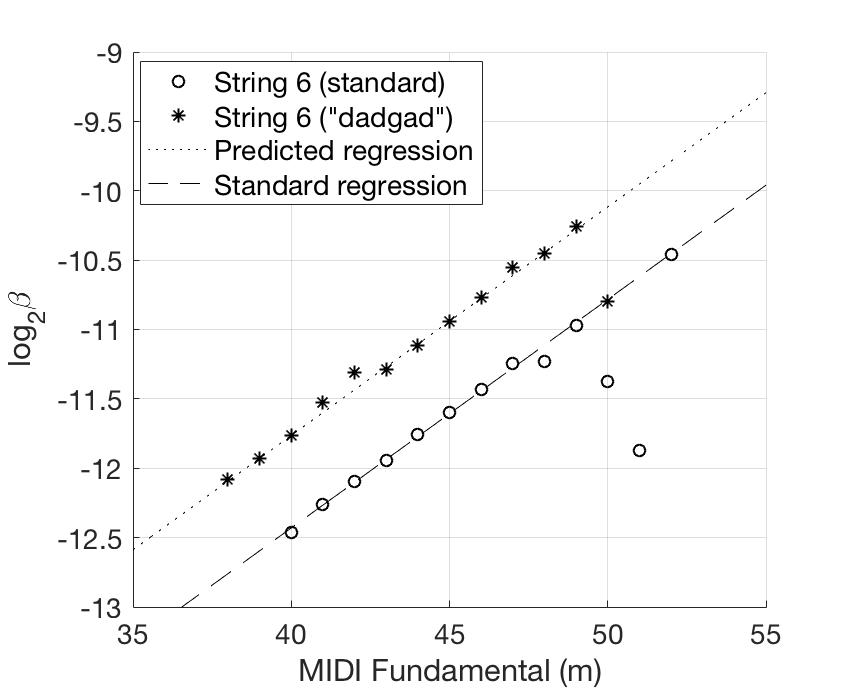
\includegraphics[scale=0.25]{tuning-eg}
%\includesvg[scale=0.25]{tuning-eg}
\caption{Effect of alternate tuning on log-inharmonicity trajectories of an electric guitar. The circles are log-inharmonicity estimates of Frets 0-12 on String 6 of RWC Electric Guitar EG131 in standard tuning, and the dashed line is their bisquare-weighted regression. The asterisks are log-inharmonicity estimates for the same frets, string, and guitar recorded two semitones down. The dotted line passing through them is the \textit{predicted} regression obtained by applying equation~\eqref{eq:3.20} to the dashed line.}
\end{figure}

\section{Results}  
\subsection{RWC Transcription}
We evaluated our baseline and regression methods using a subset of the Real World Corpus (RWC) database \citep{goto2003}. We transcribed nine RWC guitars (three classical, three acoustic, and three electric) at three levels of context which form the headings of Table~\ref{tab:error-results-RWC}: guitar-specific, guitar-averaged, and guitar-independent. For guitar-specific trials, we trained and tested the system on the same guitar using three-fold cross-validation with test folds that were one-third of the guitar recordings. For guitar-averaged trials, we trained the system on all recordings of the two guitars in the same class as the test guitar, as well as a two-thirds training portion of the test guitar, and then evaluated on the remaining third of the test guitar recordings. For guitar-independent trials, we trained the system on two of the guitars in the same class as the test guitar, and tested on all recordings of the remaining one. In all cases, Table~\ref{tab:error-results-RWC} reports error probabilities.
%\twocolumn[
%\maketitle

We performed paired-sample $t$-tests ($\alpha = 0.05$) to assess the significance of the differences in transcription error rates between our methods and the existing PCT method. Because we did not have access to the trial-by-trial transcription results of PCT, we approximated the standard deviation $\sigma_d$ of the distribution of the differences by the square root of the average of the variances of the methods $\sigma_d = \sqrt{(\sigma^2_1+\sigma^2_2)/2}$ according to the Bernoulli approximation, in which $\sigma_x^2 = p_x(1-p_x)$ and the success parameter $p_x$ is simply the difference of $1$ and the reported error probability of method $x$, i.e. $p_x = 1-\mu_x$. We calculated the $t$-score of each comparison according to $t = \mu_d/(\sigma_d/\sqrt{n})$, with $n= 78$ notes $\times 12$ recordings $=936$ classified instances over which the error probabilities were averaged ($n=468$ for the fewer recordings of the electric guitars, $n=2808$ for the overall error measures by guitar type, and $n=7020$ for the total overall error measures). Table~\ref{tab:ttest-RWC} shows a subset of Table~\ref{tab:error-results-RWC} in which significantly different transcription error rates are highlighted in gray.

\begin{figure}[!htbp]
\centering
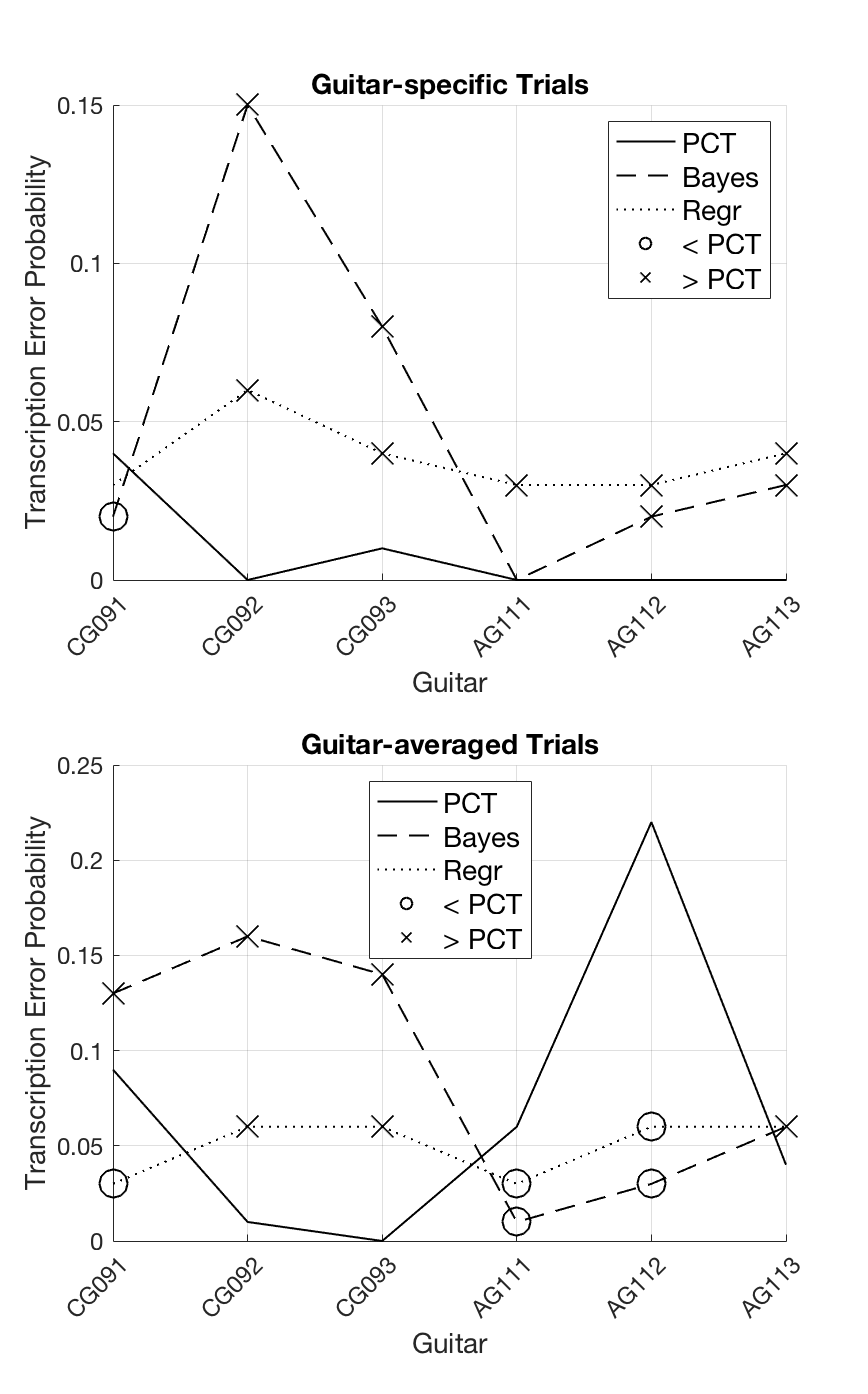
\includegraphics[scale=0.25]{sig-comp-PCT}
\caption{Error probability comparisons. Results from our baseline (``Bayes") and regression (``Regr.") methods which differ from PCT to a statistically-significant ($\alpha=0.05$) degree are shaded in gray. Electric guitar trials and ``Guitar-independent" scenarios are omitted since comparisons in those cases are not available.}
\label{tab:ttest-RWC}
\end{figure}

We next performed two-tailed McNemar test on results of our two novel methods to assess the significance ($\alpha = 0.05$) of differences in transcription error rate between them. See Table~\ref{tab:mcnemar-RWC}. Transcripts of the $78$ notes $\times 12$ recordings $= 936$ string assignments of our two classifiers for each evaluation guitar ($468$ assignments for the fewer recordings of the electric guitars, $2808$ for the overall performance by guitar type, and $7020$ for the total overall performance) along with their true labels were examined.

\begin{figure}[!htbp]
\centering
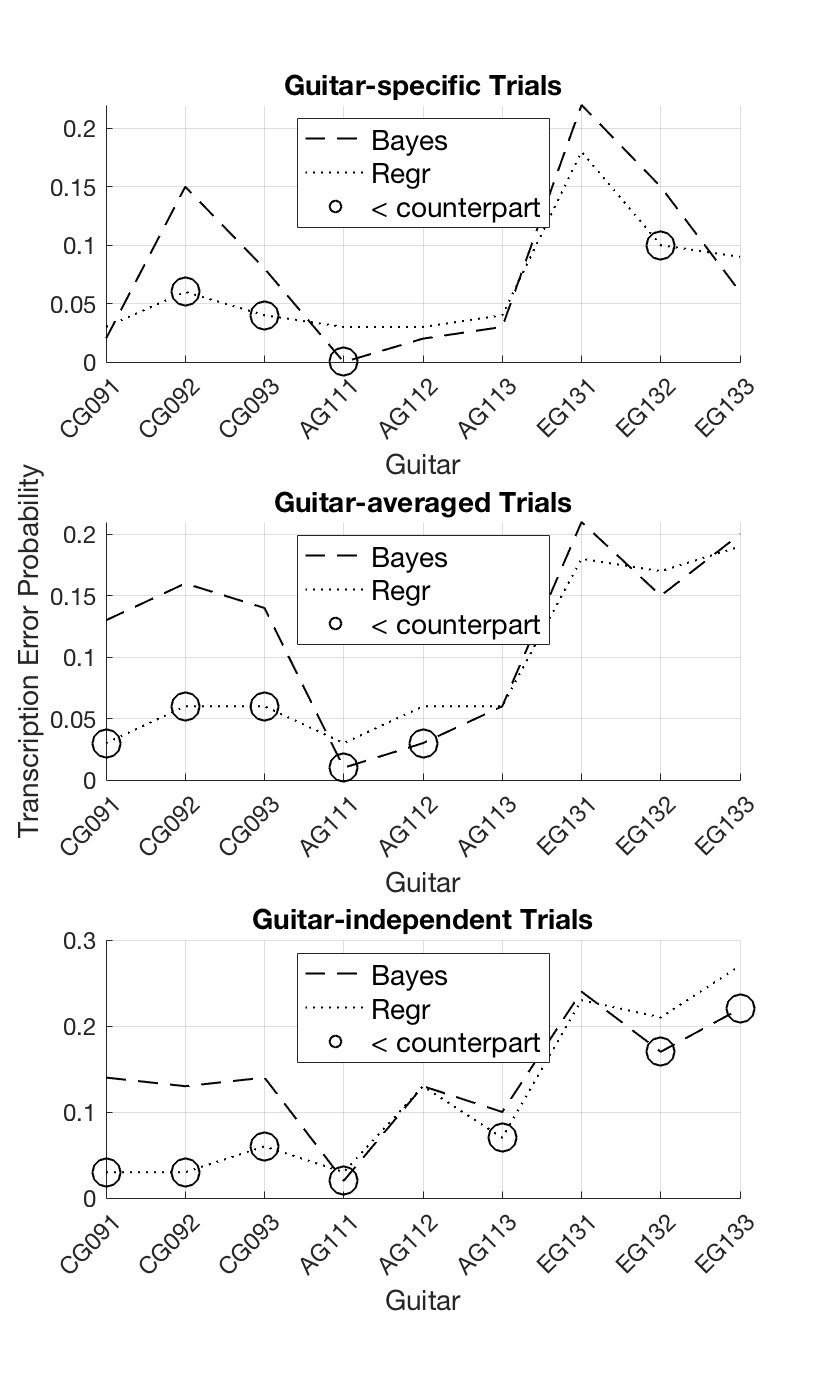
\includegraphics[scale=0.275]{novel-methods-sig-comp}
\caption{Error probability comparisons. Superior results in trials with statistically-significant ($\alpha=0.05$) performance differences are shaded in gray. PCT results omitted to highlight performance differences between our baseline and regression methods.}
\label{tab:mcnemar-RWC}
\end{figure}

\subsection{Tuning Compensation}
We evaluated our tuning compensation method on personal recordings of an electric and acoustic guitar. The string gauge of the acoustic guitar was 0.12 inches, while that of the electric guitar was unknown. We captured various tunings: standard, ``DADGAD" (in which the open pitches of String 6 through String 1 are given by the respective letters in name), ``WSU" (whole-step up), and ``WSD" (whole-step down). The electric guitar, which was recorded direct-input, was performed with a thick plectrum at center pickup orientation (both bridge and neck pickups engaged) and at similar moderate dynamic levels throughout. We recorded the acoustic guitar in an isolated chamber with a large diaphragm condenser microphone placed 12 inches away from the twelfth fret, and we also played it with a thick plectrum and at constant dynamic levels.

We learned inharmonicity regressions from the recordings of the standard-tuned RWC electric and acoustic guitar recordings, and predicted string classes on our respective recorded guitars. We evaluated string-wise F1-score performance both with and without our tuning compensation factor. In Tables~\ref{tab:resultsTune} and~\ref{tab:results-ag-tune}, compensated results are denoted by the ``comp." column, and original results without compensation are denoted by the ``orig." column.  For reference we also report transcription performance in standard tuning under the "Standard" column. We highlight in gray the results which were determined by a McNemar test to be statistically significant ($\alpha = 0.05$): highlighted `orig.' cells indicate that the performance degradation due to the corresponding tuning is significantly different from the standard-tuned performance, while highlighted `comp.' cells indicate that the performance gain achieved by our compensation system is significant with respect to its uncompensated counterpart.

\begin{table*}[!htbp]
\begin{center}
\begin{tabular}{||c||c||c|c||c|c||c|c||}
\hline
\multicolumn{8}{|c|}{\bf{Alternate-tuning Transcription F1-scores (Electric)}} \\
\hline
& Standard & \multicolumn{2}{|c|}{``DADGAD"} & \multicolumn{2}{|c|}{``WSU"} & \multicolumn{2}{|c|}{``WSD"} \\
\hline
String No. & orig. & orig. & comp. & orig. & comp. & orig. & comp. \\
\hline
1 & 0.96 & 0.96 & 0.96 & 0.87 & 0.96 & 0.96 & 0.96 \\
\hline
2 & 0.96 & 0.92 & 0.92 & 0.70 & 0.96 & 0.96 & 0.96\\
\hline
3 & 0.50 & 0.48 & 0.43 & 0.65 & 0.50 & 0.50 & 0.50\\
\hline
4 & 0.76 & 0.76 & 0.74 & 0.38 & 0.76 & 0.76 & 0.76 \\
\hline
5 & 1.00 & 1.00 & 0.87 & 0.56 & 1.00 & 1.00 & 1.00 \\
\hline
6 & 1.00 & 1.00 & 1.00 & 1.00 & 1.00 & 1.00 & 1.00\\ 
\hline
\hline
Overall: & 0.86 & 0.85 & 0.82 &  \cellcolor[gray]{0.8}0.69 & \cellcolor[gray]{0.8}0.86 & 0.86 & 0.86\\
\hline
\end{tabular}
\caption{String-wise F1-scores for our Fender Telecaster at various tunings. Regressions trained on recordings of all three RWC electric guitars. WSU: whole-step up (from standard); WSD: whole-step down (from standard); orig.: no tuning compensation used in this trial; comp.: tuning compensation used in this trial. The ``Overall" row displays average F1-score of each column. Statistically significant ($\alpha=0.05$) results highlighted in gray.} 
\label{tab:resultsTune}
\end{center}
\end{table*}

\begin{table*}[!htbp]
\begin{center}
\begin{tabular}{||c||c||c|c||c|c||c|c||}
\hline
\multicolumn{8}{|c|}{\bf{Alternate-tuning Transcription F1-scores (Acoustic)}} \\
\hline
& Standard & \multicolumn{2}{|c|}{``DADGAD"} & \multicolumn{2}{|c|}{``WSU"} & \multicolumn{2}{|c|}{``WSD"} \\
\hline
String No. & orig. & orig. & comp. & orig. & comp. & orig. & comp. \\
\hline
1 & 0.96 & 0.87 & 0.92 & 0.96 & 0.96 & 0.92 & 0.96 \\
\hline
2 & 0.82 & 0.70 & 0.63 & 0.44 & 0.82 & 0.67 & 0.92\\
\hline
3 & 0.96 & 0.93 & 1.00 & 0.74 & 0.96 & 0.00 & 0.96\\
\hline
4 & 0.87 & 0.79 & 0.79 & 0.90 & 0.87 & 0.44 & 0.93 \\
\hline
5 & 1.00 & 1.00 & 1.00 & 0.82 & 1.00 & 0.81 & 1.00 \\
\hline
6 & 1.00 & 1.00 & 1.00 & 0.96 & 1.00 & 1.00 & 1.00\\ 
\hline
\hline
Overall: & 0.93 & 0.88 & 0.89 & \cellcolor[gray]{0.8}0.80 & \cellcolor[gray]{0.8}0.93 & \cellcolor[gray]{0.8}0.64 & \cellcolor[gray]{0.8}0.96\\
\hline
\end{tabular}
\caption{String-wise F1-scores for our Takamine G-series at various tunings. Regressions trained on all recordings of all three RWC acoustic guitars. WSU: whole-step up (from standard); WSD: whole-step down (from standard); orig.: no tuning compensation used in this trial; comp.: tuning compensation used in this trial. The ``Overall" row displays average F1-score of each column. Statistically significant ($\alpha=0.05$) results highlighted in gray.} 
\label{tab:results-ag-tune}
\end{center}
\end{table*}


\section{Discussion} 
\subsection{RWC Transcription}
In Table~\ref{tab:ttest-RWC}, statistically significant differences at the $\alpha = 0.05$ level between the existing PCT method and our method show that for aggregated performance of classical and acoustic guitars (the ``Overall CG, AG" row), PCT retains ``Guitar-specific" superiority but is overtaken by our regression method in the ``Guitar-averaged" category. This suggests that there is merit to leveraging the linear structure of log-inharmonicity trajectories for improved generalized transcription. Our regression method outperforms PCT for all ``Guitar-averaged" acoustic guitars, though performs worse than PCT for classical guitars in the same scenario.

Comparison of our regression-based classifier results (``Regr." columns) and our baseline classifier results (``Bayes" columns) in Table~\ref{tab:mcnemar-RWC} revealed that leveraging the linear structure of log-inharmonicities yielded statistically significant ($\alpha = 0.05$) performance gains over the baseline method when considering overall performance of the three RWC guitar types. Interestingly, our regression method on average outperformed the baseline only for classical guitars for all headings, while the baseline mostly outperformed the the regression for only acoustic guitars. Performance on just electrics was fairly evenly split, with the regression method excelling under the ``Guitar-specific" heading, the baseline excelling under the ``Guitar-independent" heading, and no significant difference under the ``Guitar-averaged heading."

The robustness of inharmonicity-based transcription systems can be affected by phenomena which physically determine with the notes being transcribed. One such factor is guitar string geometry. We recorded identical note plucks on personal guitars exhibiting an array of combinations of string age, intonation length, gauge size, and winding, and we observed that variations in the latter two affected our log-inharmonicity measurements by orders of magnitude between one-tenth and one. The degree of this variability is commensurate with that of the log-inharmonicities of adjacent strings. The RWC database does not annotate string geometry parameters for any of its guitars, so this dimension may be partly interfering with the quality of transcription results.

\subsection{Tuning Compensation}
The alternate-tuning experiments validated our tuning compensation feature, as we see in Tables~\ref{tab:resultsTune} and~\ref{tab:results-ag-tune} that the effect of appropriately scaling the inharmonicity regressions for tunings which significantly degraded standard-tuned performance is to restore transcription accuracy towards that obtained using standard tuning. Interestingly, the effect of various tunings (``DADGAD" in both electric and acoustic, ``WSD" in the electric) on our guitars' transcriptions is statistically insignificant, suggesting that we may have overestimated how problematic some alternate tunings are for inharmonicity-based systems. Surprisingly, the ``Standard" and ``WSD" accuracies for our electric guitar are identical both with and without tuning compensation.

\section{Summary} 
Tablature is a popular music notation for guitarists because it uniquely specifies fretboard positions for musical passages. Its manual annotation process, however, is tedious. Automatic transcription systems offer a solution to this difficulty. Inharmonicity, which affects the degree of upward skew of the partials of a note, is a key feature used in some successful systems. We proposed to capitalize on the predictable log-inharmonicity trajectory of a string by characterizing it as a linear regression against its pitch, and we developed a baseline Bayesian classifier to contextualize the performance of this regression approach. Finally, we derived an inharmonicity adjustment factor that could be used to compensate for guitars recorded in alternate tunings.

Comparisons of our baseline and regression approaches against the existing PCT method revealed that, overall, the regression method achieves lower error rates when transcribing guitars on which it was not individually trained. It also outperformed our baseline, suggesting that leveraging inharmonicity trajectories is a worthwhile pursuit. We also validated our inharmonicity compensation feature, reporting accuracy increases on personal recordings of alternately-tuned electric and acoustic guitars.

\bibliographystyle{jaes}

% Reference to bibliography file.
\bibliography{mybib}


\end{document}